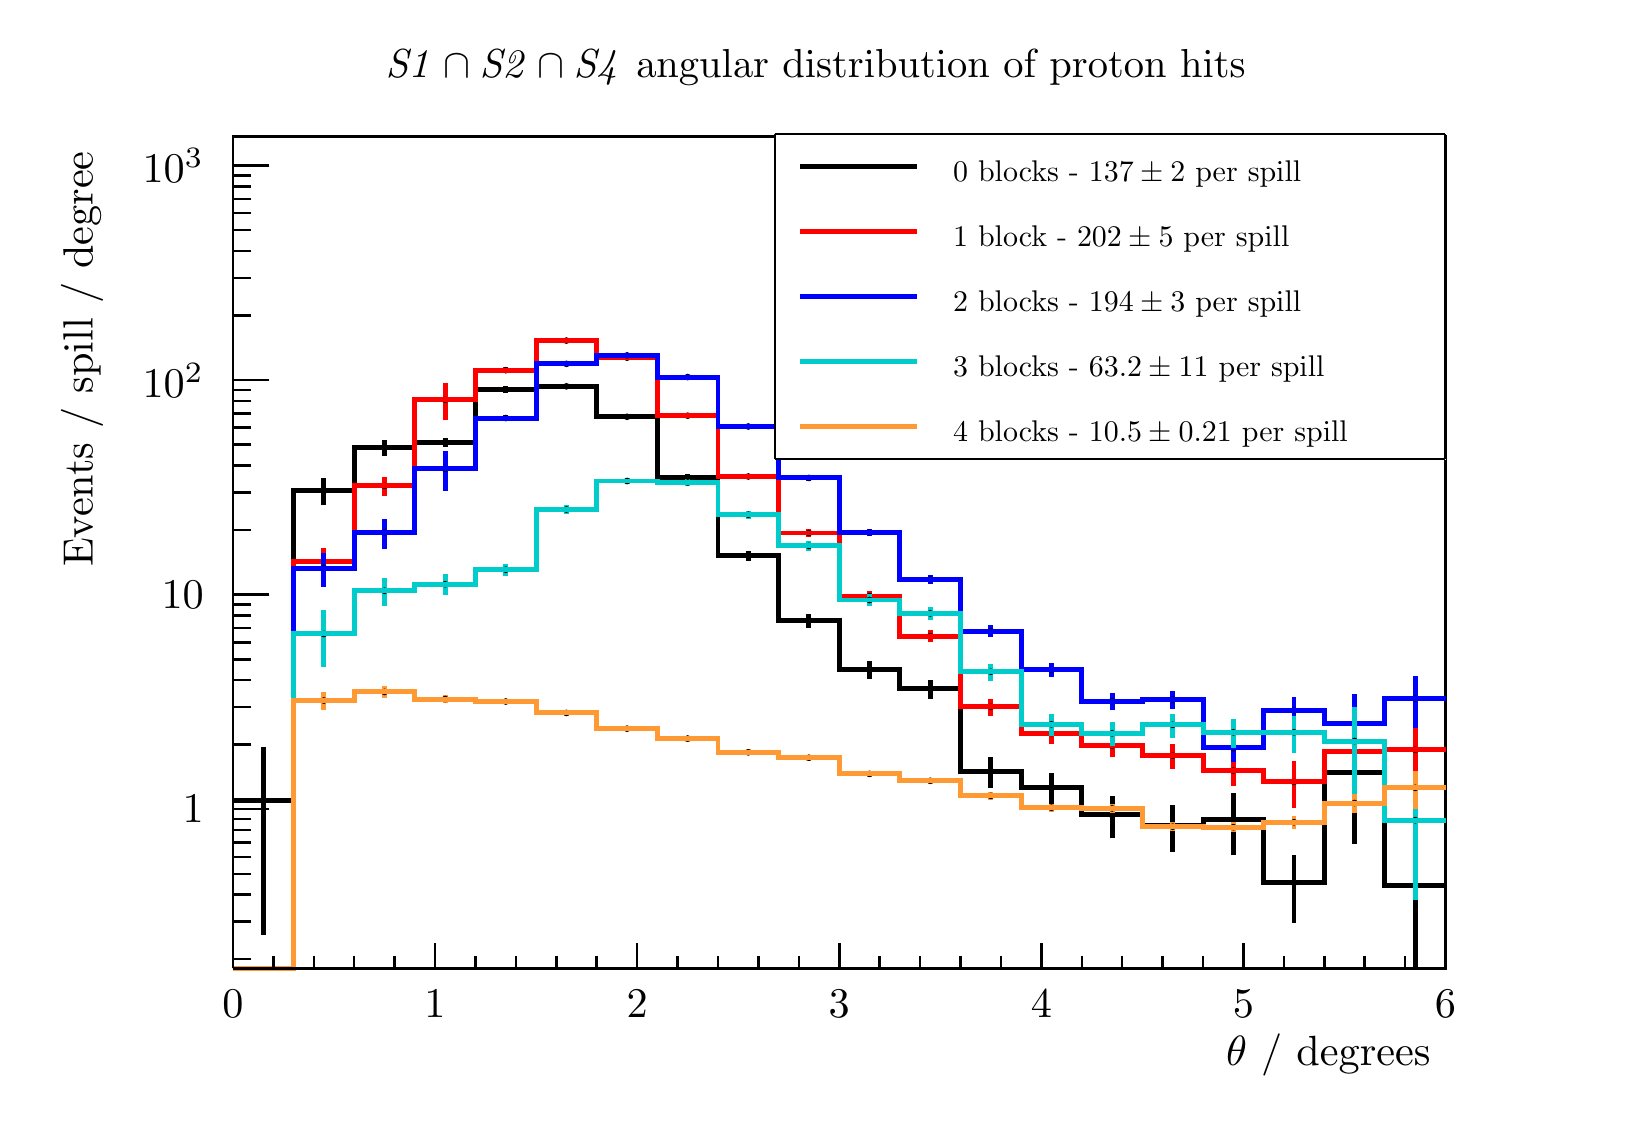
\begin{tikzpicture}
\pgfdeclareplotmark{cross} {
\pgfpathmoveto{\pgfpoint{-0.3\pgfplotmarksize}{\pgfplotmarksize}}
\pgfpathlineto{\pgfpoint{+0.3\pgfplotmarksize}{\pgfplotmarksize}}
\pgfpathlineto{\pgfpoint{+0.3\pgfplotmarksize}{0.3\pgfplotmarksize}}
\pgfpathlineto{\pgfpoint{+1\pgfplotmarksize}{0.3\pgfplotmarksize}}
\pgfpathlineto{\pgfpoint{+1\pgfplotmarksize}{-0.3\pgfplotmarksize}}
\pgfpathlineto{\pgfpoint{+0.3\pgfplotmarksize}{-0.3\pgfplotmarksize}}
\pgfpathlineto{\pgfpoint{+0.3\pgfplotmarksize}{-1.\pgfplotmarksize}}
\pgfpathlineto{\pgfpoint{-0.3\pgfplotmarksize}{-1.\pgfplotmarksize}}
\pgfpathlineto{\pgfpoint{-0.3\pgfplotmarksize}{-0.3\pgfplotmarksize}}
\pgfpathlineto{\pgfpoint{-1.\pgfplotmarksize}{-0.3\pgfplotmarksize}}
\pgfpathlineto{\pgfpoint{-1.\pgfplotmarksize}{0.3\pgfplotmarksize}}
\pgfpathlineto{\pgfpoint{-0.3\pgfplotmarksize}{0.3\pgfplotmarksize}}
\pgfpathclose
\pgfusepathqstroke
}
\pgfdeclareplotmark{cross*} {
\pgfpathmoveto{\pgfpoint{-0.3\pgfplotmarksize}{\pgfplotmarksize}}
\pgfpathlineto{\pgfpoint{+0.3\pgfplotmarksize}{\pgfplotmarksize}}
\pgfpathlineto{\pgfpoint{+0.3\pgfplotmarksize}{0.3\pgfplotmarksize}}
\pgfpathlineto{\pgfpoint{+1\pgfplotmarksize}{0.3\pgfplotmarksize}}
\pgfpathlineto{\pgfpoint{+1\pgfplotmarksize}{-0.3\pgfplotmarksize}}
\pgfpathlineto{\pgfpoint{+0.3\pgfplotmarksize}{-0.3\pgfplotmarksize}}
\pgfpathlineto{\pgfpoint{+0.3\pgfplotmarksize}{-1.\pgfplotmarksize}}
\pgfpathlineto{\pgfpoint{-0.3\pgfplotmarksize}{-1.\pgfplotmarksize}}
\pgfpathlineto{\pgfpoint{-0.3\pgfplotmarksize}{-0.3\pgfplotmarksize}}
\pgfpathlineto{\pgfpoint{-1.\pgfplotmarksize}{-0.3\pgfplotmarksize}}
\pgfpathlineto{\pgfpoint{-1.\pgfplotmarksize}{0.3\pgfplotmarksize}}
\pgfpathlineto{\pgfpoint{-0.3\pgfplotmarksize}{0.3\pgfplotmarksize}}
\pgfpathclose
\pgfusepathqfillstroke
}
\pgfdeclareplotmark{newstar} {
\pgfpathmoveto{\pgfqpoint{0pt}{\pgfplotmarksize}}
\pgfpathlineto{\pgfqpointpolar{44}{0.5\pgfplotmarksize}}
\pgfpathlineto{\pgfqpointpolar{18}{\pgfplotmarksize}}
\pgfpathlineto{\pgfqpointpolar{-20}{0.5\pgfplotmarksize}}
\pgfpathlineto{\pgfqpointpolar{-54}{\pgfplotmarksize}}
\pgfpathlineto{\pgfqpointpolar{-90}{0.5\pgfplotmarksize}}
\pgfpathlineto{\pgfqpointpolar{234}{\pgfplotmarksize}}
\pgfpathlineto{\pgfqpointpolar{198}{0.5\pgfplotmarksize}}
\pgfpathlineto{\pgfqpointpolar{162}{\pgfplotmarksize}}
\pgfpathlineto{\pgfqpointpolar{134}{0.5\pgfplotmarksize}}
\pgfpathclose
\pgfusepathqstroke
}
\pgfdeclareplotmark{newstar*} {
\pgfpathmoveto{\pgfqpoint{0pt}{\pgfplotmarksize}}
\pgfpathlineto{\pgfqpointpolar{44}{0.5\pgfplotmarksize}}
\pgfpathlineto{\pgfqpointpolar{18}{\pgfplotmarksize}}
\pgfpathlineto{\pgfqpointpolar{-20}{0.5\pgfplotmarksize}}
\pgfpathlineto{\pgfqpointpolar{-54}{\pgfplotmarksize}}
\pgfpathlineto{\pgfqpointpolar{-90}{0.5\pgfplotmarksize}}
\pgfpathlineto{\pgfqpointpolar{234}{\pgfplotmarksize}}
\pgfpathlineto{\pgfqpointpolar{198}{0.5\pgfplotmarksize}}
\pgfpathlineto{\pgfqpointpolar{162}{\pgfplotmarksize}}
\pgfpathlineto{\pgfqpointpolar{134}{0.5\pgfplotmarksize}}
\pgfpathclose
\pgfusepathqfillstroke
}
\definecolor{c}{rgb}{1,1,1};
\draw [color=c, fill=c] (0,0) rectangle (20,13.7249);
\draw [color=c, fill=c] (2.6,1.78424) rectangle (18,12.3524);
\definecolor{c}{rgb}{0,0,0};
\draw [c,line width=0.9] (2.6,1.78424) -- (2.6,12.3524) -- (18,12.3524) -- (18,1.78424) -- (2.6,1.78424);
\definecolor{c}{rgb}{1,1,1};
\draw [color=c, fill=c] (2.6,1.78424) rectangle (18,12.3524);
\definecolor{c}{rgb}{0,0,0};
\draw [c,line width=0.9] (2.6,1.78424) -- (2.6,12.3524) -- (18,12.3524) -- (18,1.78424) -- (2.6,1.78424);
\definecolor{c}{rgb}{0,0,0.6};
\draw [c,line width=0.9] (2.6,1.78424) -- (3.37,1.78424) -- (3.37,1.78424) -- (4.14,1.78424) -- (4.14,1.78424) -- (4.91,1.78424) -- (4.91,1.78424) -- (5.68,1.78424) -- (5.68,1.78424) -- (6.45,1.78424) -- (6.45,1.78424) -- (7.22,1.78424) --
 (7.22,1.78424) -- (7.99,1.78424) -- (7.99,1.78424) -- (8.76,1.78424) -- (8.76,1.78424) -- (9.53,1.78424) -- (9.53,1.78424) -- (10.3,1.78424) -- (10.3,1.78424) -- (11.07,1.78424) -- (11.07,1.78424) -- (11.84,1.78424) -- (11.84,1.78424) --
 (12.61,1.78424) -- (12.61,1.78424) -- (13.38,1.78424) -- (13.38,1.78424) -- (14.15,1.78424) -- (14.15,1.78424) -- (14.92,1.78424) -- (14.92,1.78424) -- (15.69,1.78424) -- (15.69,1.78424) -- (16.46,1.78424) -- (16.46,1.78424) -- (17.23,1.78424) --
 (17.23,1.78424) -- (18,1.78424);
\definecolor{c}{rgb}{0,0,0};
\draw [c,line width=0.9] (2.6,1.78424) -- (18,1.78424);
\draw [c,line width=0.9] (2.6,2.10129) -- (2.6,1.78424);
\draw [c,line width=0.9] (3.11333,1.94276) -- (3.11333,1.78424);
\draw [c,line width=0.9] (3.62667,1.94276) -- (3.62667,1.78424);
\draw [c,line width=0.9] (4.14,1.94276) -- (4.14,1.78424);
\draw [c,line width=0.9] (4.65333,1.94276) -- (4.65333,1.78424);
\draw [c,line width=0.9] (5.16667,2.10129) -- (5.16667,1.78424);
\draw [c,line width=0.9] (5.68,1.94276) -- (5.68,1.78424);
\draw [c,line width=0.9] (6.19333,1.94276) -- (6.19333,1.78424);
\draw [c,line width=0.9] (6.70667,1.94276) -- (6.70667,1.78424);
\draw [c,line width=0.9] (7.22,1.94276) -- (7.22,1.78424);
\draw [c,line width=0.9] (7.73333,2.10129) -- (7.73333,1.78424);
\draw [c,line width=0.9] (8.24667,1.94276) -- (8.24667,1.78424);
\draw [c,line width=0.9] (8.76,1.94276) -- (8.76,1.78424);
\draw [c,line width=0.9] (9.27333,1.94276) -- (9.27333,1.78424);
\draw [c,line width=0.9] (9.78667,1.94276) -- (9.78667,1.78424);
\draw [c,line width=0.9] (10.3,2.10129) -- (10.3,1.78424);
\draw [c,line width=0.9] (10.8133,1.94276) -- (10.8133,1.78424);
\draw [c,line width=0.9] (11.3267,1.94276) -- (11.3267,1.78424);
\draw [c,line width=0.9] (11.84,1.94276) -- (11.84,1.78424);
\draw [c,line width=0.9] (12.3533,1.94276) -- (12.3533,1.78424);
\draw [c,line width=0.9] (12.8667,2.10129) -- (12.8667,1.78424);
\draw [c,line width=0.9] (13.38,1.94276) -- (13.38,1.78424);
\draw [c,line width=0.9] (13.8933,1.94276) -- (13.8933,1.78424);
\draw [c,line width=0.9] (14.4067,1.94276) -- (14.4067,1.78424);
\draw [c,line width=0.9] (14.92,1.94276) -- (14.92,1.78424);
\draw [c,line width=0.9] (15.4333,2.10129) -- (15.4333,1.78424);
\draw [c,line width=0.9] (15.9467,1.94276) -- (15.9467,1.78424);
\draw [c,line width=0.9] (16.46,1.94276) -- (16.46,1.78424);
\draw [c,line width=0.9] (16.9733,1.94276) -- (16.9733,1.78424);
\draw [c,line width=0.9] (17.4867,1.94276) -- (17.4867,1.78424);
\draw [c,line width=0.9] (18,2.10129) -- (18,1.78424);
\draw [anchor=base] (2.6,1.16662) node[scale=1.52731, color=c, rotate=0]{0};
\draw [anchor=base] (5.16667,1.16662) node[scale=1.52731, color=c, rotate=0]{1};
\draw [anchor=base] (7.73333,1.16662) node[scale=1.52731, color=c, rotate=0]{2};
\draw [anchor=base] (10.3,1.16662) node[scale=1.52731, color=c, rotate=0]{3};
\draw [anchor=base] (12.8667,1.16662) node[scale=1.52731, color=c, rotate=0]{4};
\draw [anchor=base] (15.4333,1.16662) node[scale=1.52731, color=c, rotate=0]{5};
\draw [anchor=base] (18,1.16662) node[scale=1.52731, color=c, rotate=0]{6};
\draw [anchor= east] (18,0.686246) node[scale=1.52731, color=c, rotate=0]{$ \theta$ / degrees};
\draw [c,line width=0.9] (2.6,1.78424) -- (2.6,12.3524);
\draw [c,line width=0.9] (2.831,1.90202) -- (2.6,1.90202);
\draw [c,line width=0.9] (2.831,2.38178) -- (2.6,2.38178);
\draw [c,line width=0.9] (2.831,2.72217) -- (2.6,2.72217);
\draw [c,line width=0.9] (2.831,2.9862) -- (2.6,2.9862);
\draw [c,line width=0.9] (2.831,3.20193) -- (2.6,3.20193);
\draw [c,line width=0.9] (2.831,3.38433) -- (2.6,3.38433);
\draw [c,line width=0.9] (2.831,3.54233) -- (2.6,3.54233);
\draw [c,line width=0.9] (2.831,3.68169) -- (2.6,3.68169);
\draw [c,line width=0.9] (3.062,3.80636) -- (2.6,3.80636);
\draw [anchor= east] (2.42,3.80636) node[scale=1.52731, color=c, rotate=0]{1};
\draw [c,line width=0.9] (2.831,4.62651) -- (2.6,4.62651);
\draw [c,line width=0.9] (2.831,5.10627) -- (2.6,5.10627);
\draw [c,line width=0.9] (2.831,5.44666) -- (2.6,5.44666);
\draw [c,line width=0.9] (2.831,5.71069) -- (2.6,5.71069);
\draw [c,line width=0.9] (2.831,5.92642) -- (2.6,5.92642);
\draw [c,line width=0.9] (2.831,6.10882) -- (2.6,6.10882);
\draw [c,line width=0.9] (2.831,6.26682) -- (2.6,6.26682);
\draw [c,line width=0.9] (2.831,6.40618) -- (2.6,6.40618);
\draw [c,line width=0.9] (3.062,6.53085) -- (2.6,6.53085);
\draw [anchor= east] (2.42,6.53085) node[scale=1.52731, color=c, rotate=0]{10};
\draw [c,line width=0.9] (2.831,7.351) -- (2.6,7.351);
\draw [c,line width=0.9] (2.831,7.83076) -- (2.6,7.83076);
\draw [c,line width=0.9] (2.831,8.17115) -- (2.6,8.17115);
\draw [c,line width=0.9] (2.831,8.43518) -- (2.6,8.43518);
\draw [c,line width=0.9] (2.831,8.65091) -- (2.6,8.65091);
\draw [c,line width=0.9] (2.831,8.83331) -- (2.6,8.83331);
\draw [c,line width=0.9] (2.831,8.99131) -- (2.6,8.99131);
\draw [c,line width=0.9] (2.831,9.13067) -- (2.6,9.13067);
\draw [c,line width=0.9] (3.062,9.25534) -- (2.6,9.25534);
\draw [anchor= east] (2.42,9.25534) node[scale=1.52731, color=c, rotate=0]{$10^{2}$};
\draw [c,line width=0.9] (2.831,10.0755) -- (2.6,10.0755);
\draw [c,line width=0.9] (2.831,10.5553) -- (2.6,10.5553);
\draw [c,line width=0.9] (2.831,10.8956) -- (2.6,10.8956);
\draw [c,line width=0.9] (2.831,11.1597) -- (2.6,11.1597);
\draw [c,line width=0.9] (2.831,11.3754) -- (2.6,11.3754);
\draw [c,line width=0.9] (2.831,11.5578) -- (2.6,11.5578);
\draw [c,line width=0.9] (2.831,11.7158) -- (2.6,11.7158);
\draw [c,line width=0.9] (2.831,11.8552) -- (2.6,11.8552);
\draw [c,line width=0.9] (3.062,11.9798) -- (2.6,11.9798);
\draw [anchor= east] (2.42,11.9798) node[scale=1.52731, color=c, rotate=0]{$10^{3}$};
\draw [anchor= east] (0.683095,12.3524) node[scale=1.52731, color=c, rotate=90]{ Events / spill / degree};
\draw [c,line width=1.8] (2.985,2.2145) -- (2.985,3.92147);
\draw [c,line width=1.8] (2.985,3.92147) -- (2.985,4.59285);
\foreach \P in {(2.985,3.92147)}{\draw[mark options={color=c,fill=c},mark size=2.402402pt,mark=*,mark size=1pt] plot coordinates {\P};}
\draw [c,line width=1.8] (3.755,7.66606) -- (3.755,7.85008);
\draw [c,line width=1.8] (3.755,7.85008) -- (3.755,8.0093);
\foreach \P in {(3.755,7.85008)}{\draw[mark options={color=c,fill=c},mark size=2.402402pt,mark=*,mark size=1pt] plot coordinates {\P};}
\draw [c,line width=1.8] (4.525,8.29487) -- (4.525,8.39687);
\draw [c,line width=1.8] (4.525,8.39687) -- (4.525,8.49076);
\foreach \P in {(4.525,8.39687)}{\draw[mark options={color=c,fill=c},mark size=2.402402pt,mark=*,mark size=1pt] plot coordinates {\P};}
\draw [c,line width=1.8] (5.295,8.41105) -- (5.295,8.46905);
\draw [c,line width=1.8] (5.295,8.46905) -- (5.295,8.52434);
\foreach \P in {(5.295,8.46905)}{\draw[mark options={color=c,fill=c},mark size=2.402402pt,mark=*,mark size=1pt] plot coordinates {\P};}
\draw [c,line width=1.8] (6.065,9.09566) -- (6.065,9.13866);
\draw [c,line width=1.8] (6.065,9.13866) -- (6.065,9.18014);
\foreach \P in {(6.065,9.13866)}{\draw[mark options={color=c,fill=c},mark size=2.402402pt,mark=*,mark size=1pt] plot coordinates {\P};}
\draw [c,line width=1.8] (6.835,9.14659) -- (6.835,9.17666);
\draw [c,line width=1.8] (6.835,9.17666) -- (6.835,9.20598);
\foreach \P in {(6.835,9.17666)}{\draw[mark options={color=c,fill=c},mark size=2.402402pt,mark=*,mark size=1pt] plot coordinates {\P};}
\draw [c,line width=1.8] (7.605,8.75643) -- (7.605,8.78996);
\draw [c,line width=1.8] (7.605,8.78996) -- (7.605,8.82256);
\foreach \P in {(7.605,8.78996)}{\draw[mark options={color=c,fill=c},mark size=2.402402pt,mark=*,mark size=1pt] plot coordinates {\P};}
\draw [c,line width=1.8] (8.375,7.96941) -- (8.375,8.01437);
\draw [c,line width=1.8] (8.375,8.01437) -- (8.375,8.05768);
\foreach \P in {(8.375,8.01437)}{\draw[mark options={color=c,fill=c},mark size=2.402402pt,mark=*,mark size=1pt] plot coordinates {\P};}
\draw [c,line width=1.8] (9.145,6.96015) -- (9.145,7.02746);
\draw [c,line width=1.8] (9.145,7.02746) -- (9.145,7.09114);
\foreach \P in {(9.145,7.02746)}{\draw[mark options={color=c,fill=c},mark size=2.402402pt,mark=*,mark size=1pt] plot coordinates {\P};}
\draw [c,line width=1.8] (9.915,6.11379) -- (9.915,6.20544);
\draw [c,line width=1.8] (9.915,6.20544) -- (9.915,6.2905);
\foreach \P in {(9.915,6.20544)}{\draw[mark options={color=c,fill=c},mark size=2.402402pt,mark=*,mark size=1pt] plot coordinates {\P};}
\draw [c,line width=1.8] (10.685,5.46531) -- (10.685,5.58436);
\draw [c,line width=1.8] (10.685,5.58436) -- (10.685,5.69252);
\foreach \P in {(10.685,5.58436)}{\draw[mark options={color=c,fill=c},mark size=2.402402pt,mark=*,mark size=1pt] plot coordinates {\P};}
\draw [c,line width=1.8] (11.455,5.20895) -- (11.455,5.33717);
\draw [c,line width=1.8] (11.455,5.33717) -- (11.455,5.45284);
\foreach \P in {(11.455,5.33717)}{\draw[mark options={color=c,fill=c},mark size=2.402402pt,mark=*,mark size=1pt] plot coordinates {\P};}
\draw [c,line width=1.8] (12.225,4.08152) -- (12.225,4.28853);
\draw [c,line width=1.8] (12.225,4.28853) -- (12.225,4.46466);
\foreach \P in {(12.225,4.28853)}{\draw[mark options={color=c,fill=c},mark size=2.402402pt,mark=*,mark size=1pt] plot coordinates {\P};}
\draw [c,line width=1.8] (12.995,3.84665) -- (12.995,4.07771);
\draw [c,line width=1.8] (12.995,4.07771) -- (12.995,4.27094);
\foreach \P in {(12.995,4.07771)}{\draw[mark options={color=c,fill=c},mark size=2.402402pt,mark=*,mark size=1pt] plot coordinates {\P};}
\draw [c,line width=1.8] (13.765,3.43947) -- (13.765,3.73434);
\draw [c,line width=1.8] (13.765,3.73434) -- (13.765,3.97019);
\foreach \P in {(13.765,3.73434)}{\draw[mark options={color=c,fill=c},mark size=2.402402pt,mark=*,mark size=1pt] plot coordinates {\P};}
\draw [c,line width=1.8] (14.535,3.26448) -- (14.535,3.5955);
\draw [c,line width=1.8] (14.535,3.5955) -- (14.535,3.85387);
\foreach \P in {(14.535,3.5955)}{\draw[mark options={color=c,fill=c},mark size=2.402402pt,mark=*,mark size=1pt] plot coordinates {\P};}
\draw [c,line width=1.8] (15.305,3.22079) -- (15.305,3.67997);
\draw [c,line width=1.8] (15.305,3.67997) -- (15.305,4.00994);
\foreach \P in {(15.305,3.67997)}{\draw[mark options={color=c,fill=c},mark size=2.402402pt,mark=*,mark size=1pt] plot coordinates {\P};}
\draw [c,line width=1.8] (16.075,2.36752) -- (16.075,2.87208);
\draw [c,line width=1.8] (16.075,2.87208) -- (16.075,3.22468);
\foreach \P in {(16.075,2.87208)}{\draw[mark options={color=c,fill=c},mark size=2.402402pt,mark=*,mark size=1pt] plot coordinates {\P};}
\draw [c,line width=1.8] (16.845,3.36814) -- (16.845,4.27565);
\draw [c,line width=1.8] (16.845,4.27565) -- (16.845,4.78315);
\foreach \P in {(16.845,4.27565)}{\draw[mark options={color=c,fill=c},mark size=2.402402pt,mark=*,mark size=1pt] plot coordinates {\P};}
\draw [c,line width=1.8] (17.615,1.78424) -- (17.615,2.84284);
\draw [c,line width=1.8] (17.615,2.84284) -- (17.615,3.66726);
\foreach \P in {(17.615,2.84284)}{\draw[mark options={color=c,fill=c},mark size=2.402402pt,mark=*,mark size=1pt] plot coordinates {\P};}
\draw [c,line width=1.8] (2.6,3.92147) -- (3.37,3.92147) -- (3.37,7.85008) -- (4.14,7.85008) -- (4.14,8.39687) -- (4.91,8.39687) -- (4.91,8.46905) -- (5.68,8.46905) -- (5.68,9.13866) -- (6.45,9.13866) -- (6.45,9.17666) -- (7.22,9.17666) --
 (7.22,8.78996) -- (7.99,8.78996) -- (7.99,8.01437) -- (8.76,8.01437) -- (8.76,7.02746) -- (9.53,7.02746) -- (9.53,6.20544) -- (10.3,6.20544) -- (10.3,5.58436) -- (11.07,5.58436) -- (11.07,5.33717) -- (11.84,5.33717) -- (11.84,4.28853) --
 (12.61,4.28853) -- (12.61,4.07771) -- (13.38,4.07771) -- (13.38,3.73434) -- (14.15,3.73434) -- (14.15,3.5955) -- (14.92,3.5955) -- (14.92,3.67997) -- (15.69,3.67997) -- (15.69,2.87208) -- (16.46,2.87208) -- (16.46,4.27565) -- (17.23,4.27565) --
 (17.23,2.84284) -- (18,2.84284);
\definecolor{c}{rgb}{1,0,0};
\draw [c,line width=1.8] (3.755,6.73827) -- (3.755,6.94923);
\draw [c,line width=1.8] (3.755,6.94923) -- (3.755,7.12822);
\definecolor{c}{rgb}{0,0,0};
\foreach \P in {(3.755,6.94923)}{\draw[mark options={color=c,fill=c},mark size=2.402402pt,mark=*,mark size=1pt] plot coordinates {\P};}
\definecolor{c}{rgb}{1,0,0};
\draw [c,line width=1.8] (4.525,7.7898) -- (4.525,7.91246);
\draw [c,line width=1.8] (4.525,7.91246) -- (4.525,8.02359);
\definecolor{c}{rgb}{0,0,0};
\foreach \P in {(4.525,7.91246)}{\draw[mark options={color=c,fill=c},mark size=2.402402pt,mark=*,mark size=1pt] plot coordinates {\P};}
\definecolor{c}{rgb}{1,0,0};
\draw [c,line width=1.8] (5.295,8.74607) -- (5.295,9.00575);
\draw [c,line width=1.8] (5.295,9.00575) -- (5.295,9.21856);
\definecolor{c}{rgb}{0,0,0};
\foreach \P in {(5.295,9.00575)}{\draw[mark options={color=c,fill=c},mark size=2.402402pt,mark=*,mark size=1pt] plot coordinates {\P};}
\definecolor{c}{rgb}{1,0,0};
\draw [c,line width=1.8] (6.065,9.34282) -- (6.065,9.38231);
\draw [c,line width=1.8] (6.065,9.38231) -- (6.065,9.42052);
\definecolor{c}{rgb}{0,0,0};
\foreach \P in {(6.065,9.38231)}{\draw[mark options={color=c,fill=c},mark size=2.402402pt,mark=*,mark size=1pt] plot coordinates {\P};}
\definecolor{c}{rgb}{1,0,0};
\draw [c,line width=1.8] (6.835,9.7374) -- (6.835,9.75787);
\draw [c,line width=1.8] (6.835,9.75787) -- (6.835,9.77798);
\definecolor{c}{rgb}{0,0,0};
\foreach \P in {(6.835,9.75787)}{\draw[mark options={color=c,fill=c},mark size=2.402402pt,mark=*,mark size=1pt] plot coordinates {\P};}
\definecolor{c}{rgb}{1,0,0};
\draw [c,line width=1.8] (7.605,9.52062) -- (7.605,9.54131);
\draw [c,line width=1.8] (7.605,9.54131) -- (7.605,9.56165);
\definecolor{c}{rgb}{0,0,0};
\foreach \P in {(7.605,9.54131)}{\draw[mark options={color=c,fill=c},mark size=2.402402pt,mark=*,mark size=1pt] plot coordinates {\P};}
\definecolor{c}{rgb}{1,0,0};
\draw [c,line width=1.8] (8.375,8.77534) -- (8.375,8.80387);
\draw [c,line width=1.8] (8.375,8.80387) -- (8.375,8.83174);
\definecolor{c}{rgb}{0,0,0};
\foreach \P in {(8.375,8.80387)}{\draw[mark options={color=c,fill=c},mark size=2.402402pt,mark=*,mark size=1pt] plot coordinates {\P};}
\definecolor{c}{rgb}{1,0,0};
\draw [c,line width=1.8] (9.145,7.99363) -- (9.145,8.03186);
\draw [c,line width=1.8] (9.145,8.03186) -- (9.145,8.06889);
\definecolor{c}{rgb}{0,0,0};
\foreach \P in {(9.145,8.03186)}{\draw[mark options={color=c,fill=c},mark size=2.402402pt,mark=*,mark size=1pt] plot coordinates {\P};}
\definecolor{c}{rgb}{1,0,0};
\draw [c,line width=1.8] (9.915,7.26499) -- (9.915,7.31426);
\draw [c,line width=1.8] (9.915,7.31426) -- (9.915,7.36156);
\definecolor{c}{rgb}{0,0,0};
\foreach \P in {(9.915,7.31426)}{\draw[mark options={color=c,fill=c},mark size=2.402402pt,mark=*,mark size=1pt] plot coordinates {\P};}
\definecolor{c}{rgb}{1,0,0};
\draw [c,line width=1.8] (10.685,6.44536) -- (10.685,6.51233);
\draw [c,line width=1.8] (10.685,6.51233) -- (10.685,6.57571);
\definecolor{c}{rgb}{0,0,0};
\foreach \P in {(10.685,6.51233)}{\draw[mark options={color=c,fill=c},mark size=2.402402pt,mark=*,mark size=1pt] plot coordinates {\P};}
\definecolor{c}{rgb}{1,0,0};
\draw [c,line width=1.8] (11.455,5.92405) -- (11.455,6.00457);
\draw [c,line width=1.8] (11.455,6.00457) -- (11.455,6.07996);
\definecolor{c}{rgb}{0,0,0};
\foreach \P in {(11.455,6.00457)}{\draw[mark options={color=c,fill=c},mark size=2.402402pt,mark=*,mark size=1pt] plot coordinates {\P};}
\definecolor{c}{rgb}{1,0,0};
\draw [c,line width=1.8] (12.225,4.99331) -- (12.225,5.10607);
\draw [c,line width=1.8] (12.225,5.10607) -- (12.225,5.20902);
\definecolor{c}{rgb}{0,0,0};
\foreach \P in {(12.225,5.10607)}{\draw[mark options={color=c,fill=c},mark size=2.402402pt,mark=*,mark size=1pt] plot coordinates {\P};}
\definecolor{c}{rgb}{1,0,0};
\draw [c,line width=1.8] (12.995,4.63822) -- (12.995,4.7734);
\draw [c,line width=1.8] (12.995,4.7734) -- (12.995,4.89472);
\definecolor{c}{rgb}{0,0,0};
\foreach \P in {(12.995,4.7734)}{\draw[mark options={color=c,fill=c},mark size=2.402402pt,mark=*,mark size=1pt] plot coordinates {\P};}
\definecolor{c}{rgb}{1,0,0};
\draw [c,line width=1.8] (13.765,4.46816) -- (13.765,4.61283);
\draw [c,line width=1.8] (13.765,4.61283) -- (13.765,4.74173);
\definecolor{c}{rgb}{0,0,0};
\foreach \P in {(13.765,4.61283)}{\draw[mark options={color=c,fill=c},mark size=2.402402pt,mark=*,mark size=1pt] plot coordinates {\P};}
\definecolor{c}{rgb}{1,0,0};
\draw [c,line width=1.8] (14.535,4.32152) -- (14.535,4.48572);
\draw [c,line width=1.8] (14.535,4.48572) -- (14.535,4.62988);
\definecolor{c}{rgb}{0,0,0};
\foreach \P in {(14.535,4.48572)}{\draw[mark options={color=c,fill=c},mark size=2.402402pt,mark=*,mark size=1pt] plot coordinates {\P};}
\definecolor{c}{rgb}{1,0,0};
\draw [c,line width=1.8] (15.305,4.10119) -- (15.305,4.2972);
\draw [c,line width=1.8] (15.305,4.2972) -- (15.305,4.46531);
\definecolor{c}{rgb}{0,0,0};
\foreach \P in {(15.305,4.2972)}{\draw[mark options={color=c,fill=c},mark size=2.402402pt,mark=*,mark size=1pt] plot coordinates {\P};}
\definecolor{c}{rgb}{1,0,0};
\draw [c,line width=1.8] (16.075,3.81903) -- (16.075,4.15311);
\draw [c,line width=1.8] (16.075,4.15311) -- (16.075,4.41334);
\definecolor{c}{rgb}{0,0,0};
\foreach \P in {(16.075,4.15311)}{\draw[mark options={color=c,fill=c},mark size=2.402402pt,mark=*,mark size=1pt] plot coordinates {\P};}
\definecolor{c}{rgb}{1,0,0};
\draw [c,line width=1.8] (16.845,3.84997) -- (16.845,4.53881);
\draw [c,line width=1.8] (16.845,4.53881) -- (16.845,4.97134);
\definecolor{c}{rgb}{0,0,0};
\foreach \P in {(16.845,4.53881)}{\draw[mark options={color=c,fill=c},mark size=2.402402pt,mark=*,mark size=1pt] plot coordinates {\P};}
\definecolor{c}{rgb}{1,0,0};
\draw [c,line width=1.8] (17.615,3.8321) -- (17.615,4.56083);
\draw [c,line width=1.8] (17.615,4.56083) -- (17.615,5.00848);
\definecolor{c}{rgb}{0,0,0};
\foreach \P in {(17.615,4.56083)}{\draw[mark options={color=c,fill=c},mark size=2.402402pt,mark=*,mark size=1pt] plot coordinates {\P};}
\definecolor{c}{rgb}{1,0,0};
\draw [c,line width=1.8] (2.6,1.78424) -- (3.37,1.78424) -- (3.37,6.94923) -- (4.14,6.94923) -- (4.14,7.91246) -- (4.91,7.91246) -- (4.91,9.00575) -- (5.68,9.00575) -- (5.68,9.38231) -- (6.45,9.38231) -- (6.45,9.75787) -- (7.22,9.75787) --
 (7.22,9.54131) -- (7.99,9.54131) -- (7.99,8.80387) -- (8.76,8.80387) -- (8.76,8.03186) -- (9.53,8.03186) -- (9.53,7.31426) -- (10.3,7.31426) -- (10.3,6.51233) -- (11.07,6.51233) -- (11.07,6.00457) -- (11.84,6.00457) -- (11.84,5.10607) --
 (12.61,5.10607) -- (12.61,4.7734) -- (13.38,4.7734) -- (13.38,4.61283) -- (14.15,4.61283) -- (14.15,4.48572) -- (14.92,4.48572) -- (14.92,4.2972) -- (15.69,4.2972) -- (15.69,4.15311) -- (16.46,4.15311) -- (16.46,4.53881) -- (17.23,4.53881) --
 (17.23,4.56083) -- (18,4.56083);
\definecolor{c}{rgb}{0,0,1};
\draw [c,line width=1.8] (3.755,6.62914) -- (3.755,6.86744);
\draw [c,line width=1.8] (3.755,6.86744) -- (3.755,7.06569);
\definecolor{c}{rgb}{0,0,0};
\foreach \P in {(3.755,6.86744)}{\draw[mark options={color=c,fill=c},mark size=2.402402pt,mark=*,mark size=1pt] plot coordinates {\P};}
\definecolor{c}{rgb}{0,0,1};
\draw [c,line width=1.8] (4.525,7.11458) -- (4.525,7.32085);
\draw [c,line width=1.8] (4.525,7.32085) -- (4.525,7.49645);
\definecolor{c}{rgb}{0,0,0};
\foreach \P in {(4.525,7.32085)}{\draw[mark options={color=c,fill=c},mark size=2.402402pt,mark=*,mark size=1pt] plot coordinates {\P};}
\definecolor{c}{rgb}{0,0,1};
\draw [c,line width=1.8] (5.295,7.84877) -- (5.295,8.12732);
\draw [c,line width=1.8] (5.295,8.12732) -- (5.295,8.35263);
\definecolor{c}{rgb}{0,0,0};
\foreach \P in {(5.295,8.12732)}{\draw[mark options={color=c,fill=c},mark size=2.402402pt,mark=*,mark size=1pt] plot coordinates {\P};}
\definecolor{c}{rgb}{0,0,1};
\draw [c,line width=1.8] (6.065,8.73047) -- (6.065,8.77427);
\draw [c,line width=1.8] (6.065,8.77427) -- (6.065,8.8165);
\definecolor{c}{rgb}{0,0,0};
\foreach \P in {(6.065,8.77427)}{\draw[mark options={color=c,fill=c},mark size=2.402402pt,mark=*,mark size=1pt] plot coordinates {\P};}
\definecolor{c}{rgb}{0,0,1};
\draw [c,line width=1.8] (6.835,9.43969) -- (6.835,9.4623);
\draw [c,line width=1.8] (6.835,9.4623) -- (6.835,9.48449);
\definecolor{c}{rgb}{0,0,0};
\foreach \P in {(6.835,9.4623)}{\draw[mark options={color=c,fill=c},mark size=2.402402pt,mark=*,mark size=1pt] plot coordinates {\P};}
\definecolor{c}{rgb}{0,0,1};
\draw [c,line width=1.8] (7.605,9.54958) -- (7.605,9.56966);
\draw [c,line width=1.8] (7.605,9.56966) -- (7.605,9.58941);
\definecolor{c}{rgb}{0,0,0};
\foreach \P in {(7.605,9.56966)}{\draw[mark options={color=c,fill=c},mark size=2.402402pt,mark=*,mark size=1pt] plot coordinates {\P};}
\definecolor{c}{rgb}{0,0,1};
\draw [c,line width=1.8] (8.375,9.27077) -- (8.375,9.29454);
\draw [c,line width=1.8] (8.375,9.29454) -- (8.375,9.31785);
\definecolor{c}{rgb}{0,0,0};
\foreach \P in {(8.375,9.29454)}{\draw[mark options={color=c,fill=c},mark size=2.402402pt,mark=*,mark size=1pt] plot coordinates {\P};}
\definecolor{c}{rgb}{0,0,1};
\draw [c,line width=1.8] (9.145,8.63664) -- (9.145,8.66698);
\draw [c,line width=1.8] (9.145,8.66698) -- (9.145,8.69657);
\definecolor{c}{rgb}{0,0,0};
\foreach \P in {(9.145,8.66698)}{\draw[mark options={color=c,fill=c},mark size=2.402402pt,mark=*,mark size=1pt] plot coordinates {\P};}
\definecolor{c}{rgb}{0,0,1};
\draw [c,line width=1.8] (9.915,7.97611) -- (9.915,8.01383);
\draw [c,line width=1.8] (9.915,8.01383) -- (9.915,8.05037);
\definecolor{c}{rgb}{0,0,0};
\foreach \P in {(9.915,8.01383)}{\draw[mark options={color=c,fill=c},mark size=2.402402pt,mark=*,mark size=1pt] plot coordinates {\P};}
\definecolor{c}{rgb}{0,0,1};
\draw [c,line width=1.8] (10.685,7.27148) -- (10.685,7.32038);
\draw [c,line width=1.8] (10.685,7.32038) -- (10.685,7.36733);
\definecolor{c}{rgb}{0,0,0};
\foreach \P in {(10.685,7.32038)}{\draw[mark options={color=c,fill=c},mark size=2.402402pt,mark=*,mark size=1pt] plot coordinates {\P};}
\definecolor{c}{rgb}{0,0,1};
\draw [c,line width=1.8] (11.455,6.66654) -- (11.455,6.72644);
\draw [c,line width=1.8] (11.455,6.72644) -- (11.455,6.78346);
\definecolor{c}{rgb}{0,0,0};
\foreach \P in {(11.455,6.72644)}{\draw[mark options={color=c,fill=c},mark size=2.402402pt,mark=*,mark size=1pt] plot coordinates {\P};}
\definecolor{c}{rgb}{0,0,1};
\draw [c,line width=1.8] (12.225,5.99196) -- (12.225,6.06916);
\draw [c,line width=1.8] (12.225,6.06916) -- (12.225,6.14162);
\definecolor{c}{rgb}{0,0,0};
\foreach \P in {(12.225,6.06916)}{\draw[mark options={color=c,fill=c},mark size=2.402402pt,mark=*,mark size=1pt] plot coordinates {\P};}
\definecolor{c}{rgb}{0,0,1};
\draw [c,line width=1.8] (12.995,5.4826) -- (12.995,5.5789);
\draw [c,line width=1.8] (12.995,5.5789) -- (12.995,5.66794);
\definecolor{c}{rgb}{0,0,0};
\foreach \P in {(12.995,5.5789)}{\draw[mark options={color=c,fill=c},mark size=2.402402pt,mark=*,mark size=1pt] plot coordinates {\P};}
\definecolor{c}{rgb}{0,0,1};
\draw [c,line width=1.8] (13.765,5.06278) -- (13.765,5.17846);
\draw [c,line width=1.8] (13.765,5.17846) -- (13.765,5.28384);
\definecolor{c}{rgb}{0,0,0};
\foreach \P in {(13.765,5.17846)}{\draw[mark options={color=c,fill=c},mark size=2.402402pt,mark=*,mark size=1pt] plot coordinates {\P};}
\definecolor{c}{rgb}{0,0,1};
\draw [c,line width=1.8] (14.535,5.07962) -- (14.535,5.20012);
\draw [c,line width=1.8] (14.535,5.20012) -- (14.535,5.30948);
\definecolor{c}{rgb}{0,0,0};
\foreach \P in {(14.535,5.20012)}{\draw[mark options={color=c,fill=c},mark size=2.402402pt,mark=*,mark size=1pt] plot coordinates {\P};}
\definecolor{c}{rgb}{0,0,1};
\draw [c,line width=1.8] (15.305,4.40869) -- (15.305,4.58399);
\draw [c,line width=1.8] (15.305,4.58399) -- (15.305,4.73664);
\definecolor{c}{rgb}{0,0,0};
\foreach \P in {(15.305,4.58399)}{\draw[mark options={color=c,fill=c},mark size=2.402402pt,mark=*,mark size=1pt] plot coordinates {\P};}
\definecolor{c}{rgb}{0,0,1};
\draw [c,line width=1.8] (16.075,4.86565) -- (16.075,5.05965);
\draw [c,line width=1.8] (16.075,5.05965) -- (16.075,5.22628);
\definecolor{c}{rgb}{0,0,0};
\foreach \P in {(16.075,5.05965)}{\draw[mark options={color=c,fill=c},mark size=2.402402pt,mark=*,mark size=1pt] plot coordinates {\P};}
\definecolor{c}{rgb}{0,0,1};
\draw [c,line width=1.8] (16.845,4.3562) -- (16.845,4.8975);
\draw [c,line width=1.8] (16.845,4.8975) -- (16.845,5.2675);
\definecolor{c}{rgb}{0,0,0};
\foreach \P in {(16.845,4.8975)}{\draw[mark options={color=c,fill=c},mark size=2.402402pt,mark=*,mark size=1pt] plot coordinates {\P};}
\definecolor{c}{rgb}{0,0,1};
\draw [c,line width=1.8] (17.615,4.83284) -- (17.615,5.21034);
\draw [c,line width=1.8] (17.615,5.21034) -- (17.615,5.49609);
\definecolor{c}{rgb}{0,0,0};
\foreach \P in {(17.615,5.21034)}{\draw[mark options={color=c,fill=c},mark size=2.402402pt,mark=*,mark size=1pt] plot coordinates {\P};}
\definecolor{c}{rgb}{0,0,1};
\draw [c,line width=1.8] (2.6,1.78424) -- (3.37,1.78424) -- (3.37,6.86744) -- (4.14,6.86744) -- (4.14,7.32085) -- (4.91,7.32085) -- (4.91,8.12732) -- (5.68,8.12732) -- (5.68,8.77427) -- (6.45,8.77427) -- (6.45,9.4623) -- (7.22,9.4623) --
 (7.22,9.56966) -- (7.99,9.56966) -- (7.99,9.29454) -- (8.76,9.29454) -- (8.76,8.66698) -- (9.53,8.66698) -- (9.53,8.01383) -- (10.3,8.01383) -- (10.3,7.32038) -- (11.07,7.32038) -- (11.07,6.72644) -- (11.84,6.72644) -- (11.84,6.06916) --
 (12.61,6.06916) -- (12.61,5.5789) -- (13.38,5.5789) -- (13.38,5.17846) -- (14.15,5.17846) -- (14.15,5.20012) -- (14.92,5.20012) -- (14.92,4.58399) -- (15.69,4.58399) -- (15.69,5.05965) -- (16.46,5.05965) -- (16.46,4.8975) -- (17.23,4.8975) --
 (17.23,5.21034) -- (18,5.21034);
\definecolor{c}{rgb}{0,0.8,0.8};
\draw [c,line width=1.8] (3.755,5.61522) -- (3.755,6.03195);
\draw [c,line width=1.8] (3.755,6.03195) -- (3.755,6.33953);
\definecolor{c}{rgb}{0,0,0};
\foreach \P in {(3.755,6.03195)}{\draw[mark options={color=c,fill=c},mark size=2.402402pt,mark=*,mark size=1pt] plot coordinates {\P};}
\definecolor{c}{rgb}{0,0.8,0.8};
\draw [c,line width=1.8] (4.525,6.39049) -- (4.525,6.581);
\draw [c,line width=1.8] (4.525,6.581) -- (4.525,6.74504);
\definecolor{c}{rgb}{0,0,0};
\foreach \P in {(4.525,6.581)}{\draw[mark options={color=c,fill=c},mark size=2.402402pt,mark=*,mark size=1pt] plot coordinates {\P};}
\definecolor{c}{rgb}{0,0.8,0.8};
\draw [c,line width=1.8] (5.295,6.52386) -- (5.295,6.66305);
\draw [c,line width=1.8] (5.295,6.66305) -- (5.295,6.78757);
\definecolor{c}{rgb}{0,0,0};
\foreach \P in {(5.295,6.66305)}{\draw[mark options={color=c,fill=c},mark size=2.402402pt,mark=*,mark size=1pt] plot coordinates {\P};}
\definecolor{c}{rgb}{0,0.8,0.8};
\draw [c,line width=1.8] (6.065,6.76632) -- (6.065,6.84828);
\draw [c,line width=1.8] (6.065,6.84828) -- (6.065,6.92492);
\definecolor{c}{rgb}{0,0,0};
\foreach \P in {(6.065,6.84828)}{\draw[mark options={color=c,fill=c},mark size=2.402402pt,mark=*,mark size=1pt] plot coordinates {\P};}
\definecolor{c}{rgb}{0,0.8,0.8};
\draw [c,line width=1.8] (6.835,7.55675) -- (6.835,7.61238);
\draw [c,line width=1.8] (6.835,7.61238) -- (6.835,7.66551);
\definecolor{c}{rgb}{0,0,0};
\foreach \P in {(6.835,7.61238)}{\draw[mark options={color=c,fill=c},mark size=2.402402pt,mark=*,mark size=1pt] plot coordinates {\P};}
\definecolor{c}{rgb}{0,0.8,0.8};
\draw [c,line width=1.8] (7.605,7.93206) -- (7.605,7.9746);
\draw [c,line width=1.8] (7.605,7.9746) -- (7.605,8.01567);
\definecolor{c}{rgb}{0,0,0};
\foreach \P in {(7.605,7.9746)}{\draw[mark options={color=c,fill=c},mark size=2.402402pt,mark=*,mark size=1pt] plot coordinates {\P};}
\definecolor{c}{rgb}{0,0.8,0.8};
\draw [c,line width=1.8] (8.375,7.91223) -- (8.375,7.95688);
\draw [c,line width=1.8] (8.375,7.95688) -- (8.375,7.9999);
\definecolor{c}{rgb}{0,0,0};
\foreach \P in {(8.375,7.95688)}{\draw[mark options={color=c,fill=c},mark size=2.402402pt,mark=*,mark size=1pt] plot coordinates {\P};}
\definecolor{c}{rgb}{0,0.8,0.8};
\draw [c,line width=1.8] (9.145,7.49041) -- (9.145,7.54611);
\draw [c,line width=1.8] (9.145,7.54611) -- (9.145,7.5993);
\definecolor{c}{rgb}{0,0,0};
\foreach \P in {(9.145,7.54611)}{\draw[mark options={color=c,fill=c},mark size=2.402402pt,mark=*,mark size=1pt] plot coordinates {\P};}
\definecolor{c}{rgb}{0,0.8,0.8};
\draw [c,line width=1.8] (9.915,7.08619) -- (9.915,7.15003);
\draw [c,line width=1.8] (9.915,7.15003) -- (9.915,7.21061);
\definecolor{c}{rgb}{0,0,0};
\foreach \P in {(9.915,7.15003)}{\draw[mark options={color=c,fill=c},mark size=2.402402pt,mark=*,mark size=1pt] plot coordinates {\P};}
\definecolor{c}{rgb}{0,0.8,0.8};
\draw [c,line width=1.8] (10.685,6.38412) -- (10.685,6.46328);
\draw [c,line width=1.8] (10.685,6.46328) -- (10.685,6.53747);
\definecolor{c}{rgb}{0,0,0};
\foreach \P in {(10.685,6.46328)}{\draw[mark options={color=c,fill=c},mark size=2.402402pt,mark=*,mark size=1pt] plot coordinates {\P};}
\definecolor{c}{rgb}{0,0.8,0.8};
\draw [c,line width=1.8] (11.455,6.21066) -- (11.455,6.29311);
\draw [c,line width=1.8] (11.455,6.29311) -- (11.455,6.37018);
\definecolor{c}{rgb}{0,0,0};
\foreach \P in {(11.455,6.29311)}{\draw[mark options={color=c,fill=c},mark size=2.402402pt,mark=*,mark size=1pt] plot coordinates {\P};}
\definecolor{c}{rgb}{0,0.8,0.8};
\draw [c,line width=1.8] (12.225,5.44037) -- (12.225,5.55222);
\draw [c,line width=1.8] (12.225,5.55222) -- (12.225,5.6544);
\definecolor{c}{rgb}{0,0,0};
\foreach \P in {(12.225,5.55222)}{\draw[mark options={color=c,fill=c},mark size=2.402402pt,mark=*,mark size=1pt] plot coordinates {\P};}
\definecolor{c}{rgb}{0,0.8,0.8};
\draw [c,line width=1.8] (12.995,4.73682) -- (12.995,4.88406);
\draw [c,line width=1.8] (12.995,4.88406) -- (12.995,5.01499);
\definecolor{c}{rgb}{0,0,0};
\foreach \P in {(12.995,4.88406)}{\draw[mark options={color=c,fill=c},mark size=2.402402pt,mark=*,mark size=1pt] plot coordinates {\P};}
\definecolor{c}{rgb}{0,0.8,0.8};
\draw [c,line width=1.8] (13.765,4.60819) -- (13.765,4.76968);
\draw [c,line width=1.8] (13.765,4.76968) -- (13.765,4.91175);
\definecolor{c}{rgb}{0,0,0};
\foreach \P in {(13.765,4.76968)}{\draw[mark options={color=c,fill=c},mark size=2.402402pt,mark=*,mark size=1pt] plot coordinates {\P};}
\definecolor{c}{rgb}{0,0.8,0.8};
\draw [c,line width=1.8] (14.535,4.71688) -- (14.535,4.87836);
\draw [c,line width=1.8] (14.535,4.87836) -- (14.535,5.02042);
\definecolor{c}{rgb}{0,0,0};
\foreach \P in {(14.535,4.87836)}{\draw[mark options={color=c,fill=c},mark size=2.402402pt,mark=*,mark size=1pt] plot coordinates {\P};}
\definecolor{c}{rgb}{0,0.8,0.8};
\draw [c,line width=1.8] (15.305,4.58578) -- (15.305,4.78268);
\draw [c,line width=1.8] (15.305,4.78268) -- (15.305,4.95145);
\definecolor{c}{rgb}{0,0,0};
\foreach \P in {(15.305,4.78268)}{\draw[mark options={color=c,fill=c},mark size=2.402402pt,mark=*,mark size=1pt] plot coordinates {\P};}
\definecolor{c}{rgb}{0,0.8,0.8};
\draw [c,line width=1.8] (16.075,4.52633) -- (16.075,4.78308);
\draw [c,line width=1.8] (16.075,4.78308) -- (16.075,4.99393);
\definecolor{c}{rgb}{0,0,0};
\foreach \P in {(16.075,4.78308)}{\draw[mark options={color=c,fill=c},mark size=2.402402pt,mark=*,mark size=1pt] plot coordinates {\P};}
\definecolor{c}{rgb}{0,0.8,0.8};
\draw [c,line width=1.8] (16.845,3.99905) -- (16.845,4.67214);
\draw [c,line width=1.8] (16.845,4.67214) -- (16.845,5.09851);
\definecolor{c}{rgb}{0,0,0};
\foreach \P in {(16.845,4.67214)}{\draw[mark options={color=c,fill=c},mark size=2.402402pt,mark=*,mark size=1pt] plot coordinates {\P};}
\definecolor{c}{rgb}{0,0.8,0.8};
\draw [c,line width=1.8] (17.615,2.65135) -- (17.615,3.66683);
\draw [c,line width=1.8] (17.615,3.66683) -- (17.615,4.20514);
\definecolor{c}{rgb}{0,0,0};
\foreach \P in {(17.615,3.66683)}{\draw[mark options={color=c,fill=c},mark size=2.402402pt,mark=*,mark size=1pt] plot coordinates {\P};}
\definecolor{c}{rgb}{0,0.8,0.8};
\draw [c,line width=1.8] (2.6,1.78424) -- (3.37,1.78424) -- (3.37,6.03195) -- (4.14,6.03195) -- (4.14,6.581) -- (4.91,6.581) -- (4.91,6.66305) -- (5.68,6.66305) -- (5.68,6.84828) -- (6.45,6.84828) -- (6.45,7.61238) -- (7.22,7.61238) -- (7.22,7.9746)
 -- (7.99,7.9746) -- (7.99,7.95688) -- (8.76,7.95688) -- (8.76,7.54611) -- (9.53,7.54611) -- (9.53,7.15003) -- (10.3,7.15003) -- (10.3,6.46328) -- (11.07,6.46328) -- (11.07,6.29311) -- (11.84,6.29311) -- (11.84,5.55222) -- (12.61,5.55222) --
 (12.61,4.88406) -- (13.38,4.88406) -- (13.38,4.76968) -- (14.15,4.76968) -- (14.15,4.87836) -- (14.92,4.87836) -- (14.92,4.78268) -- (15.69,4.78268) -- (15.69,4.78308) -- (16.46,4.78308) -- (16.46,4.67214) -- (17.23,4.67214) -- (17.23,3.66683) --
 (18,3.66683);
\definecolor{c}{rgb}{1,0.6,0.2};
\draw [c,line width=1.8] (3.755,5.06336) -- (3.755,5.18646);
\draw [c,line width=1.8] (3.755,5.18646) -- (3.755,5.29794);
\definecolor{c}{rgb}{0,0,0};
\foreach \P in {(3.755,5.18646)}{\draw[mark options={color=c,fill=c},mark size=2.402402pt,mark=*,mark size=1pt] plot coordinates {\P};}
\definecolor{c}{rgb}{1,0.6,0.2};
\draw [c,line width=1.8] (4.525,5.22165) -- (4.525,5.29595);
\draw [c,line width=1.8] (4.525,5.29595) -- (4.525,5.36586);
\definecolor{c}{rgb}{0,0,0};
\foreach \P in {(4.525,5.29595)}{\draw[mark options={color=c,fill=c},mark size=2.402402pt,mark=*,mark size=1pt] plot coordinates {\P};}
\definecolor{c}{rgb}{1,0.6,0.2};
\draw [c,line width=1.8] (5.295,5.157) -- (5.295,5.20555);
\draw [c,line width=1.8] (5.295,5.20555) -- (5.295,5.25219);
\definecolor{c}{rgb}{0,0,0};
\foreach \P in {(5.295,5.20555)}{\draw[mark options={color=c,fill=c},mark size=2.402402pt,mark=*,mark size=1pt] plot coordinates {\P};}
\definecolor{c}{rgb}{1,0.6,0.2};
\draw [c,line width=1.8] (6.065,5.13729) -- (6.065,5.17394);
\draw [c,line width=1.8] (6.065,5.17394) -- (6.065,5.2095);
\definecolor{c}{rgb}{0,0,0};
\foreach \P in {(6.065,5.17394)}{\draw[mark options={color=c,fill=c},mark size=2.402402pt,mark=*,mark size=1pt] plot coordinates {\P};}
\definecolor{c}{rgb}{1,0.6,0.2};
\draw [c,line width=1.8] (6.835,4.99291) -- (6.835,5.02946);
\draw [c,line width=1.8] (6.835,5.02946) -- (6.835,5.06492);
\definecolor{c}{rgb}{0,0,0};
\foreach \P in {(6.835,5.02946)}{\draw[mark options={color=c,fill=c},mark size=2.402402pt,mark=*,mark size=1pt] plot coordinates {\P};}
\definecolor{c}{rgb}{1,0.6,0.2};
\draw [c,line width=1.8] (7.605,4.79467) -- (7.605,4.8292);
\draw [c,line width=1.8] (7.605,4.8292) -- (7.605,4.86275);
\definecolor{c}{rgb}{0,0,0};
\foreach \P in {(7.605,4.8292)}{\draw[mark options={color=c,fill=c},mark size=2.402402pt,mark=*,mark size=1pt] plot coordinates {\P};}
\definecolor{c}{rgb}{1,0.6,0.2};
\draw [c,line width=1.8] (8.375,4.66545) -- (8.375,4.70354);
\draw [c,line width=1.8] (8.375,4.70354) -- (8.375,4.74044);
\definecolor{c}{rgb}{0,0,0};
\foreach \P in {(8.375,4.70354)}{\draw[mark options={color=c,fill=c},mark size=2.402402pt,mark=*,mark size=1pt] plot coordinates {\P};}
\definecolor{c}{rgb}{1,0.6,0.2};
\draw [c,line width=1.8] (9.145,4.48933) -- (9.145,4.52826);
\draw [c,line width=1.8] (9.145,4.52826) -- (9.145,4.56596);
\definecolor{c}{rgb}{0,0,0};
\foreach \P in {(9.145,4.52826)}{\draw[mark options={color=c,fill=c},mark size=2.402402pt,mark=*,mark size=1pt] plot coordinates {\P};}
\definecolor{c}{rgb}{1,0.6,0.2};
\draw [c,line width=1.8] (9.915,4.42107) -- (9.915,4.46051);
\draw [c,line width=1.8] (9.915,4.46051) -- (9.915,4.49868);
\definecolor{c}{rgb}{0,0,0};
\foreach \P in {(9.915,4.46051)}{\draw[mark options={color=c,fill=c},mark size=2.402402pt,mark=*,mark size=1pt] plot coordinates {\P};}
\definecolor{c}{rgb}{1,0.6,0.2};
\draw [c,line width=1.8] (10.685,4.21469) -- (10.685,4.25547);
\draw [c,line width=1.8] (10.685,4.25547) -- (10.685,4.29488);
\definecolor{c}{rgb}{0,0,0};
\foreach \P in {(10.685,4.25547)}{\draw[mark options={color=c,fill=c},mark size=2.402402pt,mark=*,mark size=1pt] plot coordinates {\P};}
\definecolor{c}{rgb}{1,0.6,0.2};
\draw [c,line width=1.8] (11.455,4.12465) -- (11.455,4.16744);
\draw [c,line width=1.8] (11.455,4.16744) -- (11.455,4.20873);
\definecolor{c}{rgb}{0,0,0};
\foreach \P in {(11.455,4.16744)}{\draw[mark options={color=c,fill=c},mark size=2.402402pt,mark=*,mark size=1pt] plot coordinates {\P};}
\definecolor{c}{rgb}{1,0.6,0.2};
\draw [c,line width=1.8] (12.225,3.92905) -- (12.225,3.97571);
\draw [c,line width=1.8] (12.225,3.97571) -- (12.225,4.02061);
\definecolor{c}{rgb}{0,0,0};
\foreach \P in {(12.225,3.97571)}{\draw[mark options={color=c,fill=c},mark size=2.402402pt,mark=*,mark size=1pt] plot coordinates {\P};}
\definecolor{c}{rgb}{1,0.6,0.2};
\draw [c,line width=1.8] (12.995,3.77479) -- (12.995,3.82515);
\draw [c,line width=1.8] (12.995,3.82515) -- (12.995,3.87345);
\definecolor{c}{rgb}{0,0,0};
\foreach \P in {(12.995,3.82515)}{\draw[mark options={color=c,fill=c},mark size=2.402402pt,mark=*,mark size=1pt] plot coordinates {\P};}
\definecolor{c}{rgb}{1,0.6,0.2};
\draw [c,line width=1.8] (13.765,3.76231) -- (13.765,3.81598);
\draw [c,line width=1.8] (13.765,3.81598) -- (13.765,3.86731);
\definecolor{c}{rgb}{0,0,0};
\foreach \P in {(13.765,3.81598)}{\draw[mark options={color=c,fill=c},mark size=2.402402pt,mark=*,mark size=1pt] plot coordinates {\P};}
\definecolor{c}{rgb}{1,0.6,0.2};
\draw [c,line width=1.8] (14.535,3.52557) -- (14.535,3.58438);
\draw [c,line width=1.8] (14.535,3.58438) -- (14.535,3.64041);
\definecolor{c}{rgb}{0,0,0};
\foreach \P in {(14.535,3.58438)}{\draw[mark options={color=c,fill=c},mark size=2.402402pt,mark=*,mark size=1pt] plot coordinates {\P};}
\definecolor{c}{rgb}{1,0.6,0.2};
\draw [c,line width=1.8] (15.305,3.51288) -- (15.305,3.5776);
\draw [c,line width=1.8] (15.305,3.5776) -- (15.305,3.63897);
\definecolor{c}{rgb}{0,0,0};
\foreach \P in {(15.305,3.5776)}{\draw[mark options={color=c,fill=c},mark size=2.402402pt,mark=*,mark size=1pt] plot coordinates {\P};}
\definecolor{c}{rgb}{1,0.6,0.2};
\draw [c,line width=1.8] (16.075,3.55574) -- (16.075,3.64093);
\draw [c,line width=1.8] (16.075,3.64093) -- (16.075,3.72041);
\definecolor{c}{rgb}{0,0,0};
\foreach \P in {(16.075,3.64093)}{\draw[mark options={color=c,fill=c},mark size=2.402402pt,mark=*,mark size=1pt] plot coordinates {\P};}
\definecolor{c}{rgb}{1,0.6,0.2};
\draw [c,line width=1.8] (16.845,3.75307) -- (16.845,3.88502);
\draw [c,line width=1.8] (16.845,3.88502) -- (16.845,4.00371);
\definecolor{c}{rgb}{0,0,0};
\foreach \P in {(16.845,3.88502)}{\draw[mark options={color=c,fill=c},mark size=2.402402pt,mark=*,mark size=1pt] plot coordinates {\P};}
\definecolor{c}{rgb}{1,0.6,0.2};
\draw [c,line width=1.8] (17.615,3.81283) -- (17.615,4.07777);
\draw [c,line width=1.8] (17.615,4.07777) -- (17.615,4.2941);
\definecolor{c}{rgb}{0,0,0};
\foreach \P in {(17.615,4.07777)}{\draw[mark options={color=c,fill=c},mark size=2.402402pt,mark=*,mark size=1pt] plot coordinates {\P};}
\definecolor{c}{rgb}{1,0.6,0.2};
\draw [c,line width=1.8] (2.6,1.78424) -- (3.37,1.78424) -- (3.37,5.18646) -- (4.14,5.18646) -- (4.14,5.29595) -- (4.91,5.29595) -- (4.91,5.20555) -- (5.68,5.20555) -- (5.68,5.17394) -- (6.45,5.17394) -- (6.45,5.02946) -- (7.22,5.02946) --
 (7.22,4.8292) -- (7.99,4.8292) -- (7.99,4.70354) -- (8.76,4.70354) -- (8.76,4.52826) -- (9.53,4.52826) -- (9.53,4.46051) -- (10.3,4.46051) -- (10.3,4.25547) -- (11.07,4.25547) -- (11.07,4.16744) -- (11.84,4.16744) -- (11.84,3.97571) --
 (12.61,3.97571) -- (12.61,3.82515) -- (13.38,3.82515) -- (13.38,3.81598) -- (14.15,3.81598) -- (14.15,3.58438) -- (14.92,3.58438) -- (14.92,3.5776) -- (15.69,3.5776) -- (15.69,3.64093) -- (16.46,3.64093) -- (16.46,3.88502) -- (17.23,3.88502) --
 (17.23,4.07777) -- (18,4.07777);
\definecolor{c}{rgb}{0,0,0};
\draw [c,line width=0.9] (2.6,1.78424) -- (18,1.78424);
\draw [c,line width=0.9] (2.6,2.10129) -- (2.6,1.78424);
\draw [c,line width=0.9] (3.11333,1.94276) -- (3.11333,1.78424);
\draw [c,line width=0.9] (3.62667,1.94276) -- (3.62667,1.78424);
\draw [c,line width=0.9] (4.14,1.94276) -- (4.14,1.78424);
\draw [c,line width=0.9] (4.65333,1.94276) -- (4.65333,1.78424);
\draw [c,line width=0.9] (5.16667,2.10129) -- (5.16667,1.78424);
\draw [c,line width=0.9] (5.68,1.94276) -- (5.68,1.78424);
\draw [c,line width=0.9] (6.19333,1.94276) -- (6.19333,1.78424);
\draw [c,line width=0.9] (6.70667,1.94276) -- (6.70667,1.78424);
\draw [c,line width=0.9] (7.22,1.94276) -- (7.22,1.78424);
\draw [c,line width=0.9] (7.73333,2.10129) -- (7.73333,1.78424);
\draw [c,line width=0.9] (8.24667,1.94276) -- (8.24667,1.78424);
\draw [c,line width=0.9] (8.76,1.94276) -- (8.76,1.78424);
\draw [c,line width=0.9] (9.27333,1.94276) -- (9.27333,1.78424);
\draw [c,line width=0.9] (9.78667,1.94276) -- (9.78667,1.78424);
\draw [c,line width=0.9] (10.3,2.10129) -- (10.3,1.78424);
\draw [c,line width=0.9] (10.8133,1.94276) -- (10.8133,1.78424);
\draw [c,line width=0.9] (11.3267,1.94276) -- (11.3267,1.78424);
\draw [c,line width=0.9] (11.84,1.94276) -- (11.84,1.78424);
\draw [c,line width=0.9] (12.3533,1.94276) -- (12.3533,1.78424);
\draw [c,line width=0.9] (12.8667,2.10129) -- (12.8667,1.78424);
\draw [c,line width=0.9] (13.38,1.94276) -- (13.38,1.78424);
\draw [c,line width=0.9] (13.8933,1.94276) -- (13.8933,1.78424);
\draw [c,line width=0.9] (14.4067,1.94276) -- (14.4067,1.78424);
\draw [c,line width=0.9] (14.92,1.94276) -- (14.92,1.78424);
\draw [c,line width=0.9] (15.4333,2.10129) -- (15.4333,1.78424);
\draw [c,line width=0.9] (15.9467,1.94276) -- (15.9467,1.78424);
\draw [c,line width=0.9] (16.46,1.94276) -- (16.46,1.78424);
\draw [c,line width=0.9] (16.9733,1.94276) -- (16.9733,1.78424);
\draw [c,line width=0.9] (17.4867,1.94276) -- (17.4867,1.78424);
\draw [c,line width=0.9] (18,2.10129) -- (18,1.78424);
\draw [c,line width=0.9] (2.6,1.78424) -- (2.6,12.3524);
\draw [c,line width=0.9] (2.831,1.90202) -- (2.6,1.90202);
\draw [c,line width=0.9] (2.831,2.38178) -- (2.6,2.38178);
\draw [c,line width=0.9] (2.831,2.72217) -- (2.6,2.72217);
\draw [c,line width=0.9] (2.831,2.9862) -- (2.6,2.9862);
\draw [c,line width=0.9] (2.831,3.20193) -- (2.6,3.20193);
\draw [c,line width=0.9] (2.831,3.38433) -- (2.6,3.38433);
\draw [c,line width=0.9] (2.831,3.54233) -- (2.6,3.54233);
\draw [c,line width=0.9] (2.831,3.68169) -- (2.6,3.68169);
\draw [c,line width=0.9] (3.062,3.80636) -- (2.6,3.80636);
\draw [c,line width=0.9] (2.831,4.62651) -- (2.6,4.62651);
\draw [c,line width=0.9] (2.831,5.10627) -- (2.6,5.10627);
\draw [c,line width=0.9] (2.831,5.44666) -- (2.6,5.44666);
\draw [c,line width=0.9] (2.831,5.71069) -- (2.6,5.71069);
\draw [c,line width=0.9] (2.831,5.92642) -- (2.6,5.92642);
\draw [c,line width=0.9] (2.831,6.10882) -- (2.6,6.10882);
\draw [c,line width=0.9] (2.831,6.26682) -- (2.6,6.26682);
\draw [c,line width=0.9] (2.831,6.40618) -- (2.6,6.40618);
\draw [c,line width=0.9] (3.062,6.53085) -- (2.6,6.53085);
\draw [c,line width=0.9] (2.831,7.351) -- (2.6,7.351);
\draw [c,line width=0.9] (2.831,7.83076) -- (2.6,7.83076);
\draw [c,line width=0.9] (2.831,8.17115) -- (2.6,8.17115);
\draw [c,line width=0.9] (2.831,8.43518) -- (2.6,8.43518);
\draw [c,line width=0.9] (2.831,8.65091) -- (2.6,8.65091);
\draw [c,line width=0.9] (2.831,8.83331) -- (2.6,8.83331);
\draw [c,line width=0.9] (2.831,8.99131) -- (2.6,8.99131);
\draw [c,line width=0.9] (2.831,9.13067) -- (2.6,9.13067);
\draw [c,line width=0.9] (3.062,9.25534) -- (2.6,9.25534);
\draw [c,line width=0.9] (2.831,10.0755) -- (2.6,10.0755);
\draw [c,line width=0.9] (2.831,10.5553) -- (2.6,10.5553);
\draw [c,line width=0.9] (2.831,10.8956) -- (2.6,10.8956);
\draw [c,line width=0.9] (2.831,11.1597) -- (2.6,11.1597);
\draw [c,line width=0.9] (2.831,11.3754) -- (2.6,11.3754);
\draw [c,line width=0.9] (2.831,11.5578) -- (2.6,11.5578);
\draw [c,line width=0.9] (2.831,11.7158) -- (2.6,11.7158);
\draw [c,line width=0.9] (2.831,11.8552) -- (2.6,11.8552);
\draw [c,line width=0.9] (3.062,11.9798) -- (2.6,11.9798);
\draw (10,13.2265) node[scale=1.46368, color=c, rotate=0]{$\mathit{S1} \cap \mathit{S2} \cap \mathit{S4}$ angular distribution of proton hits};
\definecolor{c}{rgb}{1,1,1};
\draw [color=c, fill=c] (9.48424,8.25215) rectangle (17.9943,12.3782);
\definecolor{c}{rgb}{0,0,0};
\draw [c,line width=0.9] (9.48424,8.25215) -- (17.9943,8.25215);
\draw [c,line width=0.9] (17.9943,8.25215) -- (17.9943,12.3782);
\draw [c,line width=0.9] (17.9943,12.3782) -- (9.48424,12.3782);
\draw [c,line width=0.9] (9.48424,12.3782) -- (9.48424,8.25215);
\draw [anchor=base west] (11.6117,11.7799) node[scale=1.08185, color=c, rotate=0]{0 blocks - $137 \pm 2$ per spill};
\draw [c,line width=1.8] (9.80337,11.9656) -- (11.2926,11.9656);
\draw [anchor=base west] (11.6117,10.9547) node[scale=1.08185, color=c, rotate=0]{1 block - $202 \pm 5$ per spill};
\definecolor{c}{rgb}{1,0,0};
\draw [c,line width=1.8] (9.80337,11.1404) -- (11.2926,11.1404);
\definecolor{c}{rgb}{0,0,0};
\draw [anchor=base west] (11.6117,10.1295) node[scale=1.08185, color=c, rotate=0]{2 blocks - $194 \pm 3$ per spill};
\definecolor{c}{rgb}{0,0,1};
\draw [c,line width=1.8] (9.80337,10.3152) -- (11.2926,10.3152);
\definecolor{c}{rgb}{0,0,0};
\draw [anchor=base west] (11.6117,9.3043) node[scale=1.08185, color=c, rotate=0]{3 blocks - $63.2 \pm 11$ per spill};
\definecolor{c}{rgb}{0,0.8,0.8};
\draw [c,line width=1.8] (9.80337,9.48997) -- (11.2926,9.48997);
\definecolor{c}{rgb}{0,0,0};
\draw [anchor=base west] (11.6117,8.47908) node[scale=1.08185, color=c, rotate=0]{4 blocks - $10.5 \pm 0.21$ per spill};
\definecolor{c}{rgb}{1,0.6,0.2};
\draw [c,line width=1.8] (9.80337,8.66476) -- (11.2926,8.66476);
\end{tikzpicture}
